\documentclass{article}

\usepackage{graphicx}
\usepackage{tikz}
\usepackage{tikzsymbols}
\usetikzlibrary{calc,patterns,shapes.geometric}
\pagestyle{empty}
\usepackage[margin=0pt]{geometry}
\geometry{papersize={14in,12in}}

\def\centerarc[#1](#2)(#3:#4:#5){\draw[#1] ($(#2)+({#5*cos(#3)},{#5*sin(#3)})$) arc (#3:#4:#5);}

\begin{document}
	\begin{figure}
		\centering
		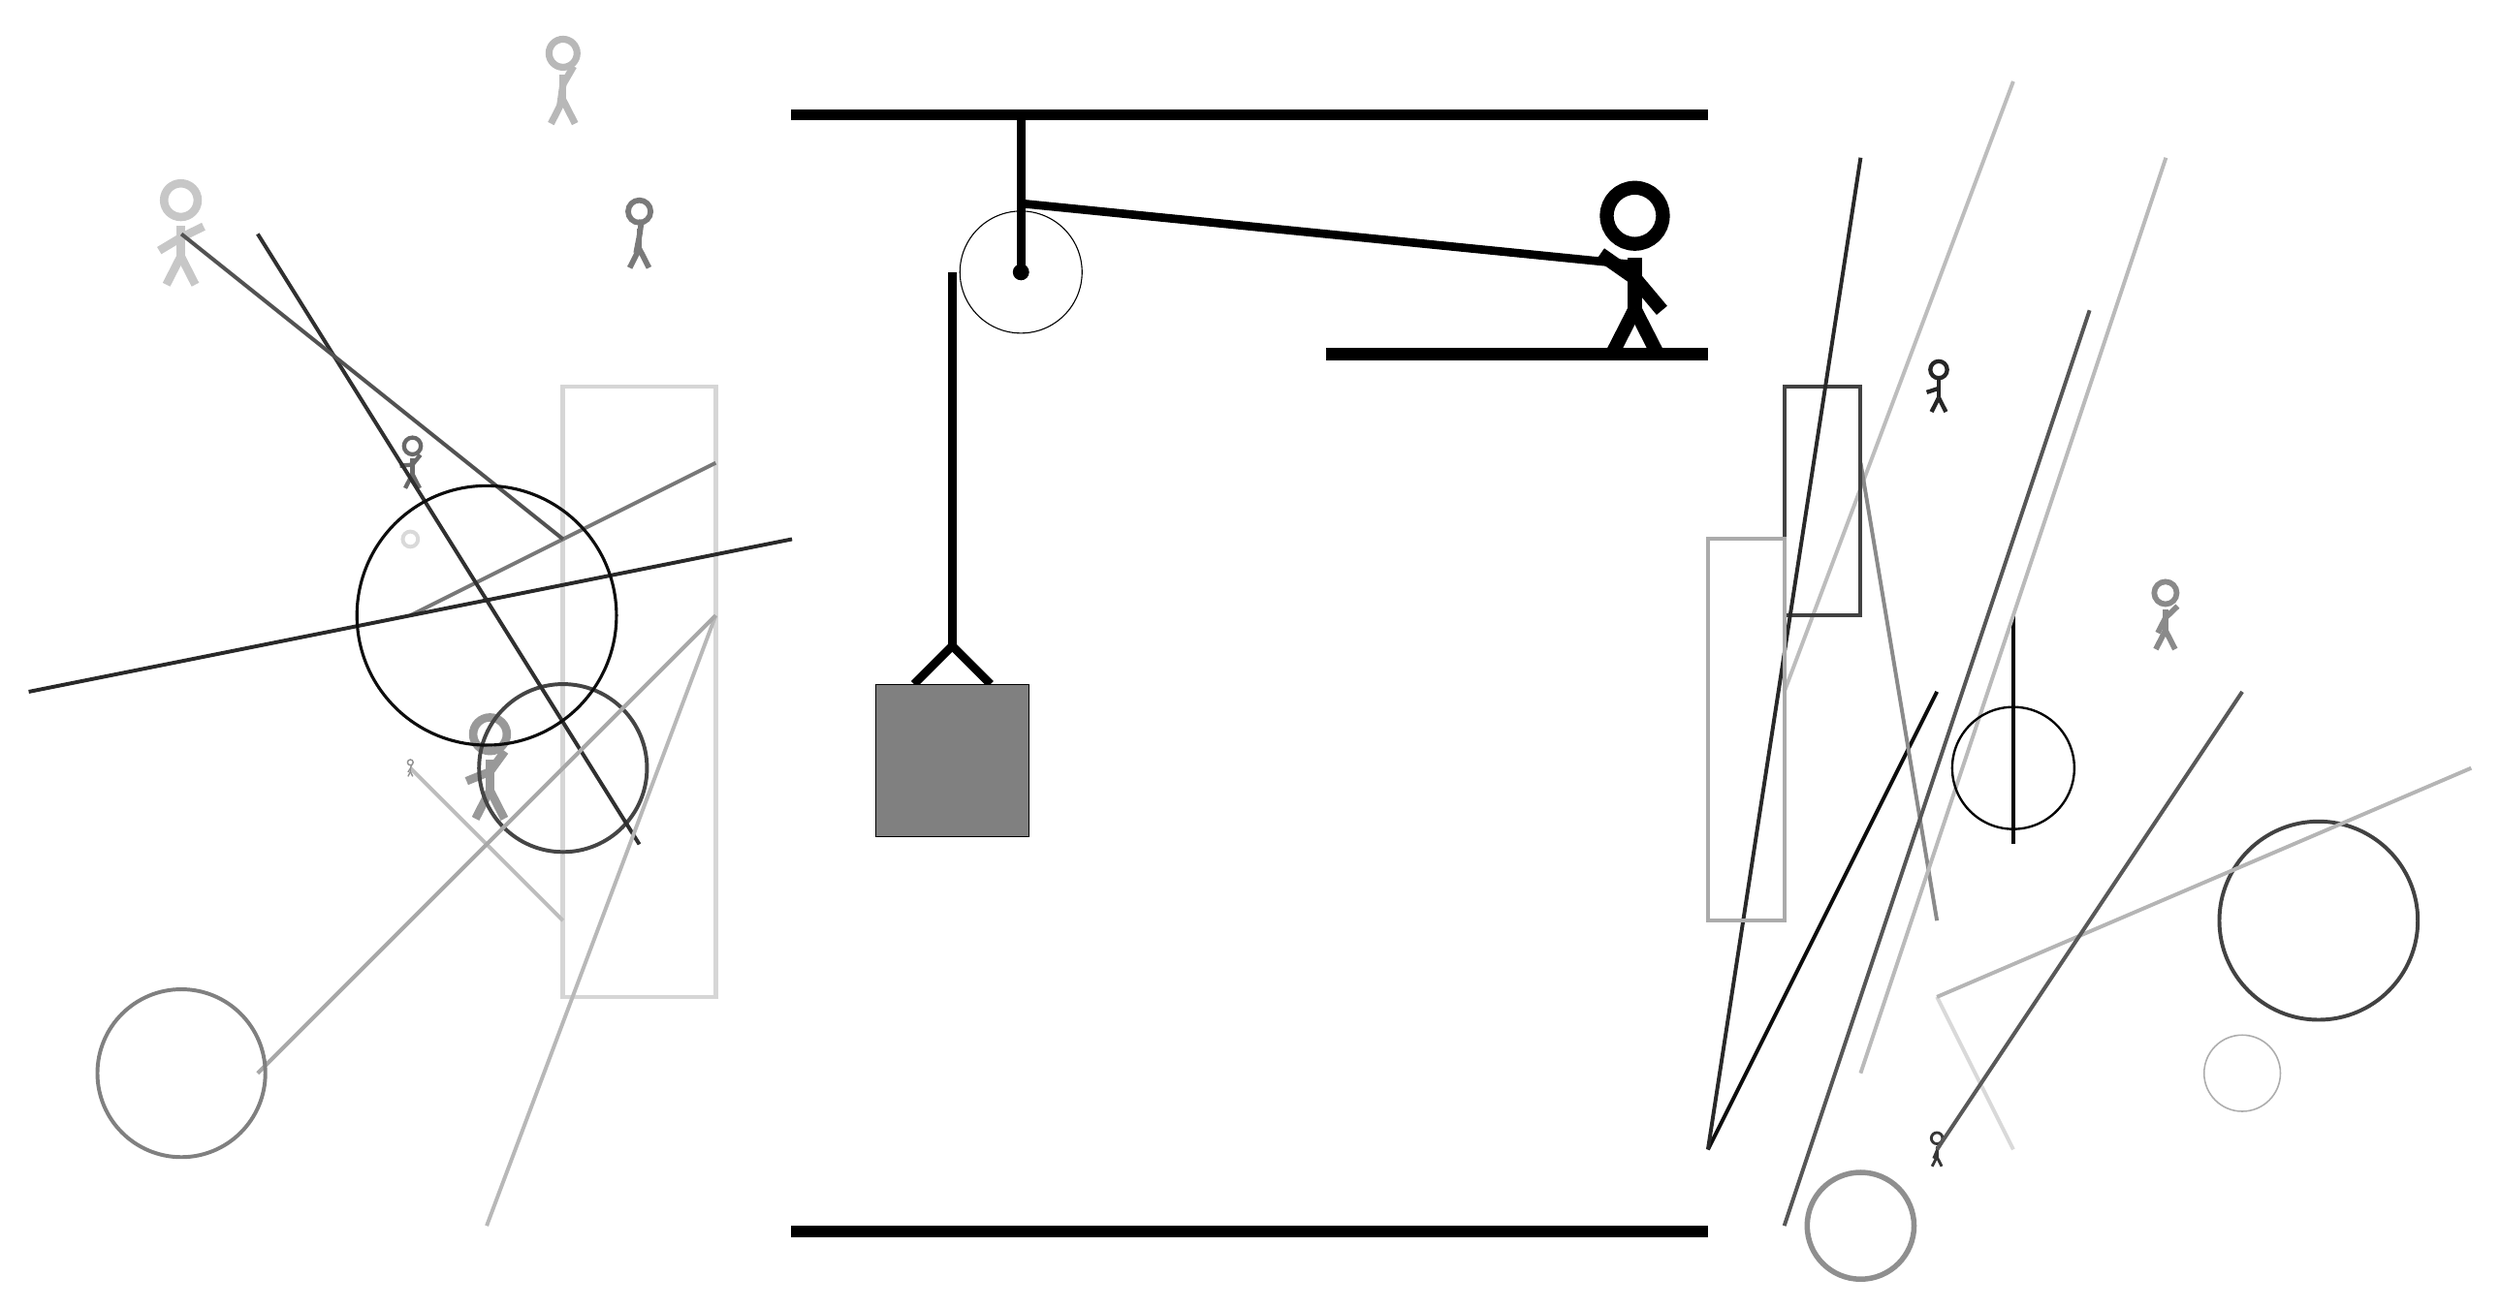
\begin{tikzpicture}
			%%%%% START %%%%%
			
			\draw[fill=black] (-2, 11.5) rectangle (10, 11.625);
			
			\draw (1, 9.5) circle (0.8);
			\draw[fill=black] (1, 9.5) circle (0.1);
			\draw[line width=1.1mm] (1, 11.5) -- (1, 9.5);
			
			\draw[line width=1.1mm](-0.4, 4.1) --  (0.1, 4.6) -- (0.6, 4.1);
			\draw[fill=black!50] (-0.9, 4.1) rectangle (1.1, 2.1);
			
			\draw[line width=1.1mm](0.1, 9.5) -- (0.1, 4.6);
			\centerarc[line width=1.1mm](1, 9.5)(90:180:0.9)
			\draw[line width=1.1mm](1, 10.4) -- (9, 9.6);
			
			\node at (9, 9.5) {\Strichmaxerl[10][-35][-50]};
			\draw[fill=black] (5, 8.5) rectangle (10, 8.35);
			
			\node[line width=0.5mm, color=black!79] at (13, -2) {\Strichmaxerl[2][67][60]};
			
			\draw[line width=0.5mm, color=black!95](13, 4) -- (10, -2);
			\draw [line width=0.2mm, color=black!32](17, -1) circle (0.5);
			\draw[line width=0.6mm, color=black!16] (-3, 8) rectangle (-5, 0);
			\node[line width=0.5mm, color=black!40] at (-6, 3) {\Strichmaxerl[6][22][54]};
			\draw [line width=0.5mm, color=black!73](-5, 3) circle (1.1);
			\draw [line width=0.5mm, color=black!74](18, 1) circle (1.3);
			
			\node[line width=0.5mm, color=black!28] at (-5, 12) {\Strichmaxerl[5][82][60]};
			\draw[line width=0.5mm, color=black!99](14, 5) -- (14, 2);
			\node[line width=0.5mm, color=black!46] at (16, 5) {\Strichmaxerl[4][63][44]};
			
			\draw [line width=0.5mm, color=black!15](-7, 6) circle (0.1);
			\draw[line width=0.5mm, color=black!53](-3, 7) -- (-7, 5);
			\draw [line width=0.7mm, color=black!44](12, -3) circle (0.7);
			
			\draw[line width=0.5mm, color=black!26](11, 4) -- (14, 12);
			\draw[line width=0.5mm, color=black!46](13, 1) -- (12, 7);
			\draw[line width=0.5mm, color=black!66](15, 9) -- (11, -3);
			\draw[line width=0.5mm, color=black!15](13, 0) -- (14, -2);
			
			\node[line width=0.2mm, color=black!22] at (-10, 10) {\Strichmaxerl[6][31][26]};
			\node[line width=0.7mm, color=black!59] at (-7, 7) {\Strichmaxerl[3][5][51]};
			\draw[line width=0.5mm, color=black!74] (12, 8) rectangle (11, 5);
			\draw[line width=0.5mm, color=black!81](-4, 2) -- (-9, 10);
			
			\draw[line width=0.5mm, color=black!26](-7, 3) -- (-5, 1);
			\draw[line width=0.5mm, color=black!28](-3, 5) -- (-6, -3);
			\draw[line width=0.5mm, color=black!84](10, -2) -- (12, 11);
			\draw[line width=0.5mm, color=black!29](13, 0) -- (20, 3);
			\draw[line width=0.5mm, color=black!27](12, -1) -- (16, 11);
			\draw[line width=0.5mm, color=black!34](-3, 5) -- (-9, -1);
			\node[line width=0.7mm, color=black!85] at (13, 8) {\Strichmaxerl[3][18][90]};
			\node[line width=0.7mm, color=black!52] at (-4, 10) {\Strichmaxerl[4][79][82]};
			\draw[line width=0.5mm, color=black!68](-5, 6) -- (-10, 10);
			\draw[line width=0.5mm, color=black!33] (11, 1) rectangle (10, 6);
			
			\draw [line width=0.3mm, color=black!99](14, 3) circle (0.8);
			\draw[line width=0.5mm, color=black!84](-2, 6) -- (-12, 4);
			\draw [line width=0.4mm, color=black!95](-6, 5) circle (1.7);
			
			\draw [line width=0.5mm, color=black!50](-10, -1) circle (1.1);
			\draw[line width=0.5mm, color=black!65](13, -2) -- (17, 4);
			
			\node[line width=0.6mm, color=black!43] at (-7, 3) {\Strichmaxerl[1][55][73]};
			
			
			\draw[fill=black] (-2, -3) rectangle (10, -3.15);
			
			%%%%% END %%%%%
		\end{tikzpicture}
	\end{figure}	
\end{document}